%-------------------------------------------------------------------------
% Design Project Input/Output Module Description
%-------------------------------------------------------------------------

\clearpage
\section{Relay Output Module}
\label{sec-output-relay}

This output module enables your IoT device to control electrical devices
such as heaters, small skillets, lights, etc. with a signal from an
Arduino. This is ideal for making controllable lights, precision timing
cooking devices, automatic shutoff water kettles and coffee roasters,
home automation projects, or for controlling any device that plugs into
the electrical wall socket.

A sample circuit and Arduino code is shown below to get you started.
First, test the example code with the relay connected to the Arduino and
\IT{not} connected to the power strip / wall socket. Power strips / wall
sockets run at a high voltage of \wu{110}{V}, so it is good practice to
test that the circuit works with the Arduino first, which runs at a much
safer voltage of \wu{3.3--5}{V}. To connect a wire to the relay pins,
ask for a small flathead screwdriver and use it to loosen tiny screws
above each pin (turn the screw counter-clockwise to loosen), which will
open tiny wire holders in the slot below. Slip the wire into the holder
and then use the screwdriver again to tighten (turn the screw clockwise
to tighten) until the wire is steady and firm. Then program the Arduino.

The example code turns the relay on and off for {5}{s} each in a loop.
After programming the Arduino, you should see the LED turn on and off
for {5}{s}. The LED indicates when the device under control is receiving
power. If this works, you can plug one end of the relay into a power
strip / wall socket, and you can plug an appliance (e.g., a mini-fan)
into the other end. Turn the fan on and make sure it is on for {5}{s}
and off for {5}{s}. Try experimenting with other devices and see what
you can control! Modify the {5}{s} looped Arduino code if you want to
control timing in other ways.

\vspace{0.1in}
\begin{minipage}[t]{0.49\tw}
  \vspace{0.0in}
  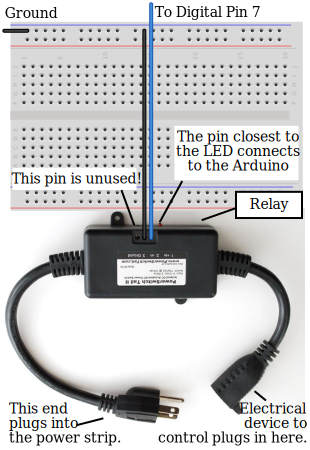
\includegraphics[width=\tw]{output-relay-annotated.svg.pdf}
\end{minipage}
\hspace{0.1in}
\begin{minipage}[t]{0.49\tw}
  \vspace{0.1in}
  \begin{Verbatim}[gobble=3,fontsize=\small]
    int pin_relay = 7;

    void setup() {
      pinMode( pin_relay, OUTPUT );
    }

    void loop() {
      digitalWrite( pin_relay, HIGH );
      delay(5000);
      digitalWrite( pin_relay, LOW );
      delay(5000);
    }
  \end{Verbatim}
\end{minipage}
\vspace{0.1in}

%Questions:
